%%%%%%%%%%%%%%%%%%%%%%%%%%%%%%%%%%%%%%%%%%%%%%%%%%%%%%%%%%%%%%%%%%%%%%%%%%%%%%%%
%2345678901234567890123456789012345678901234567890123456789012345678901234567890
%        1         2         3         4         5         6         7         8

\documentclass[letterpaper, 10 pt, conference]{ieeeconf}  
\usepackage{graphicx}


%In case you encounter the following error:
%Error 1010 The PDF file may be corrupt (unable to open PDF file) OR
%Error 1000 An error occurred while parsing a contents stream. Unable to analyze the PDF file.
%This is a known problem with pdfLaTeX conversion filter. The file cannot be opened with acrobat reader
%Please use one of the alternatives below to circumvent this error by uncommenting one or the other
%\pdfobjcompresslevel=0
%\pdfminorversion=4

% See the \addtolength command later in the file to balance the column lengths
% on the last page of the document

% The following packages can be found on http:\\www.ctan.org
%\usepackage{graphics} % for pdf, bitmapped graphics files
%\usepackage{epsfig} % for postscript graphics files
%\usepackage{mathptmx} % assumes new font selection scheme installed
%\usepackage{times} % assumes new font selection scheme installed
%\usepackage{amsmath} % assumes amsmath package installed
%\usepackage{amssymb}  % assumes amsmath package installed

\title{\LARGE \bf
Rude Robot Navigation
}


\author{Ethan Harrah, Pranav Gupta, Olamide Ogunsanya, and Anthony Tran% 
}


\begin{document}



\maketitle
\thispagestyle{empty}
\pagestyle{empty}


%%%%%%%%%%%%%%%%%%%%%%%%%%%%%%%%%%%%%%%%%%%%%%%%%%%%%%%%%%%%%%%%%%%%%%%%%%%%%%%%
\begin{abstract}
As technology progresses, there will be a need for mobile robots and humans to navigate safely within a busy traffic environment. Thus, there is a need for path planning algorithms that will help robots to pick up on the social cues that humans emit that give insight into where they are going. Gaze and head orientation are the two leading indicators used to deduce this information. This study uses renowned virtual reality technology to place participants in a simulated environment where the different paths and reactions they take to the end of the hallway in response to a robot coming at them were observed. The results of this study demonstrate the importance of head orientation as a predictive factor of someone's walking motion. Moreover, it gives insight into expected robot behavior from humans and the similarity between navigation used to get out of the robot's path. The findings of this study can be used to improve upon existing social navigation systems for mobile robots.
\end{abstract}


%%%%%%%%%%%%%%%%%%%%%%%%%%%%%%%%%%%%%%%%%%%%%%%%%%%%%%%%%%%%%%%%%%%%%%%%%%%%%%%%
\section{Introduction}
For years, researchers have sought ways to improve the social navigation of robots so that they may coexist in the same space as us [1]. People can move out of each other's way by observing specific cues that will indicate the direction they are about to turn or what path they will stick with. However, this is nearly impossible with robots as they do not give off the same social cues as humans. This makes the challenge of coexisting in the same space quite challenging. Thus, researchers have focused on developing social navigation systems that will allow them to anticipate a person's movement using specific metrics. These indicators give insight into how the robot will get out of someone's path by predicting it. Some of these measures include gaze, head orientation, and pose [2]. Prior work goes in-depth to find which cue is the first observed and the most indicative of the route a person is about to take. We took inspiration from these studies to form our approach. Rather than focusing on testing the robot and finding the best way to stay out of a person's way, we decided to test the person. In doing so, we had the robot anticipate and track a person's movements to stay in front of them and block their path. This capability is just as essential as the former because of the uses that arise from it. For example, with successful implementation, a robot would be able to deter people from entering a particular restricted area. More importantly, as in our case, it can be used to test how people react and change their trajectory in response to a robot getting in their way, rather than expecting the robot to move. 
    
    Using a tracking-based algorithm in virtual reality, we had the robot go and block a person's pathway. This paper implements a study design similar to that of a previous study that had participants go to a designated point in VR and then collect data on the most predictive indicator of where they would go [2]. However, our data centers around the different paths people will take when facing a robot coming right at them. This information is vital when trying to derive trends that may point to similarities in navigation when they see the robot coming straight for them. Observing how people react to this situation would produce stimulating results that lead to improved algorithms for social navigation. Consequently, this study makes substantial progress towards the long-term goal of both a robot and human being able to pick up on cues from each other to navigate comfortably in the same environment.

\section{Related Works}
As the first indicators of movement, previous research techniques include using obstacle positioning and velocity to predict the trajectory of an object and build a prohibited region around the projected path where the robot is not allowed to enter [3]. This methodology primarily works in environments such as hallways where there is one main direction that a person can walk but struggles in situations where there is more than one possible pathway. Another downside to the method is that human motion can be unpredictable due to unplanned stimuli such as fear [2]. In work environments such as construction sites, accidents can cause an auditory stimulus that causes a person to change their initial path and velocity suddenly. An algorithm that follows the previous methodology will not have enough time to change directions immediately or stop to readjust since tracking the previous velocity might run into the person.

An alternative indicator of motion is using a person's head orientation. Head orientation is more accurate in situations where velocity is erratic since the gaze can still predict a person's next move [4]. Researcher Lauri Nummenmaa has found that humans preemptively anticipate another person's motion by the orientation of their eyes [5]. In eye-tracking experiments, participants relied on an animated character's gaze to predict their direction. Furthermore, research by Hollands suggests that head orientation and gaze are the first two factors that occur before a person commits to a directional change [7]. In trials, saccadic eye movements are made, followed by head alignment before locomotive movement. Thus, head orientation can become a visual queue that communicates to others where one will walk before doing the actual walking.


\section{Methodology}
    We constructed a hallway and robot model in Blender and then imported it into Unity to set up the simulated environment. From there, we set up the bounds of the simulation to restrict movement within the hallway.
    To get the robot to track the participant's movements, we used C sharp to develop an algorithm that allows a robot to anticipate, track, and block a person's path dependent on where they were looking.
        The algorithm revolved around the headset's position and rotation being tracked continuously, thus placing a significant emphasis on the head orientation of the test subject.
         An invisible target is projected onto the ground as a transform of the headset. This target stays four units in front of the headset unless a wall is detected in front of the player; then, the target distance will decrease, making sure it remains 85\% of the distance to the outer walls. The robot runs on a loop, where time is constantly ticking up. If the time is below 2 seconds, the robot will perform a continuous rotation from its current forward vector to the one that points toward the tracked target. After that, for 1 second, it will perform a constant translation, where it moves from its current position to the position two units away in the direction of its normal vector. Our approach could easily be implemented outside of VR in order to get testing with actual robot models. You would only need a camera on the robot to track the targeted person's head and rotation. 

\section{Study Design}

\begin{figure}
\centering
\includegraphics[scale=0.5]{Hallway.png}
\caption{The diagram of the study in which the study takes place. The black dot is the starting point of the participant which is enclosed by the usable part of the hallway. The cube is representative of the robot that starts outside of the usable part of the hallway but inside of the virtually simulated hallway.}
\end{figure}


   The use of virtual reality in the application of human-robot interaction is on a constant incline. Through the profoundly engaging virtual reality world, there are more efficient ways to implement different systems for better experimentation. The HTC Vive Pro Eye [4], along with the respective camera headset and base stations, provided us with the ability to set up an environment in which the robot can easily track the user's movement.
   
    In this study, participants walked down a simulated hallway. The diagram of the study is presented in Figure 1, while the user's perspective in the virtual reality system can be seen in Figure 2a, and the real-world environment can be seen in Figure 2b. The dimensions of the usable part of the hallway, better known as the "play area," are 9.75 meters in length and 4.28 meters in width. Our study consisted of five different trials. Participants were told to start at the same location for each test, 2.14 meters right of the starting point and 1.22 meters forward. They were then told two main rules: to walk generally towards the end of the hallway and to never come in direct contact with the robot to better simulate a real-life environment.
    For each trial, the robot started outside the usable part of the hallway and then moved to the inside part as the test was conducted.
    
    The first three trials were conducted to create the perception in the user's mind that the robot was an ordinary machine working on going from one side of the hallway to the other side, just like the user. While the first three trials were done for testing purposes, these trials also allowed people who haven't worked with virtual reality to get more comfortable with the environment. We implemented a simple avoiding algorithm that detected if the user was in the same lane as the robot such that the robot could take the initiative to move to the opposite lane. In the first trial, the participant was told to sway left and move forward while doing the instructions above. Similarly, the participant was then instructed to sway towards the right end of the hallway and move forward in the second trial. In the third and last trial for the avoiding algorithm, the participant was told they had free will to move in any direction they wanted as long as they still followed the main rules. 
    
    The fourth consisted of the "rude" robot navigation. The head orientation of the user projected an invisible dot for the robot to track and move to use minute rotations and movement. The user was blind to the change in the robot algorithm and provided the same rules as the third trial. While there is a control in the manner of where the participants start, the movement and end location of the user is entirely dependent on them. Our purpose of creating this openness for the participant was to ultimately allow for individuality in the user's experience and consequently learn more about the interactions between humans and robots. After a hopeful while of attempting to move past the robot or reaching the end of the usable part of the hallway, we notified the user to stop and take off their headset. 
    
    
    At this point, the participant is fully aware that the robot has been programmed to track and reach the user's position. To take advantage of this state, we implemented a fifth and final trial similar to before. By doing this, we can better understand how the participants will react, knowing that the robot is targeting them. This trial is an essential step in better understanding how humans and robots will interact in areas meant to co-exist. 
    
    
    The study required using the HTC Vive Pro Eye headset and two Vive controllers. While the user did not use the controllers, they were needed for better system calibration. The hallway and the environment were implemented in Unity [11] version 2019.4.8f1 along with the help of blender [12] version 2.83. The study also applied the use of SteamVR [13] in conjunction with the HTC Vive Pro Eye headset to allow users to use the virtual reality system in the respective environment. The ability to create the play area was done by using the two SteamVR Base Station 2.0's and placing them approximately 10.5 meters away from each other. 
    
    Eleven participants ranging from 18 - 21 participated in this study. All participants in this study were unaware of the algorithms implemented within the robot's design and took place at Anna Hiss Gymnasium of the University of Texas. Permission to record was given and done using the OBS Studio software [14]. At the end of the study, each participant was asked to fill out a survey to better understand their experiences.
\begin{figure}
\centering
\includegraphics[scale=0.35]{VR Perspective.png}
\caption{The participant's virtual reality view of the robot as the simulation is started. The participants are instructed to avoid contact with the robot while attempting to reach the end of the hallway.}
\end{figure}
    
\section{Results}
For trials 1, 2, and 3, the robot avoided the participants, so head orientation was primarily focused on the end of the hallway. For trials 4 and 5, when the robot started to block the participants, their head orientation focused more on the robot than at the end of the hallway. 

When faced with the incoming robot, 100\% of participants first stopped to figure out an appropriate change of course and then changed their gaze very quickly to embark on another path.

All but one of the participants stated that the first three trials impacted their movement strategy when the robot began to come after them. They indicated that they had become lax and assumed that the robot was designed to stay out of their way. Thus, they started to walk normally until the 4th trial arrived.

On average, it took participants 5-6 seconds to figure out that the robot was following them, and they had to adjust accordingly. Many of them were shocked by the sudden change and started to look in different directions to find a way to get past the robot. About 82\% of participants took a "zig-zag" approach in which they switched up their path and head orientation erratically. The other 2 participants simply sped up their pace and walked fast to outrun the robot. 



\addtolength{\textheight}{-12cm}   % This command serves to balance the column lengths
                                  % on the last page of the document manually. It shortens
                                  % the textheight of the last page by a suitable amount.
                                  % This command does not take effect until the next page
                                  % so it should come on the page before the last. Make
                                  % sure that you do not shorten the textheight too much.

%%%%%%%%%%%%%%%%%%%%%%%%%%%%%%%%%%%%%%%%%%%%%%%%%%%%%%%%%%%%%%%%%%%%%%%%%%%%%%%%



%%%%%%%%%%%%%%%%%%%%%%%%%%%%%%%%%%%%%%%%%%%%%%%%%%%%%%%%%%%%%%%%%%%%%%%%%%%%%%%%



%%%%%%%%%%%%%%%%%%%%%%%%%%%%%%%%%%%%%%%%%%%%%%%%%%%%%%%%%%%%%%%%%%%%%%%%%%%%%%%%

\begin{figure}
\centering
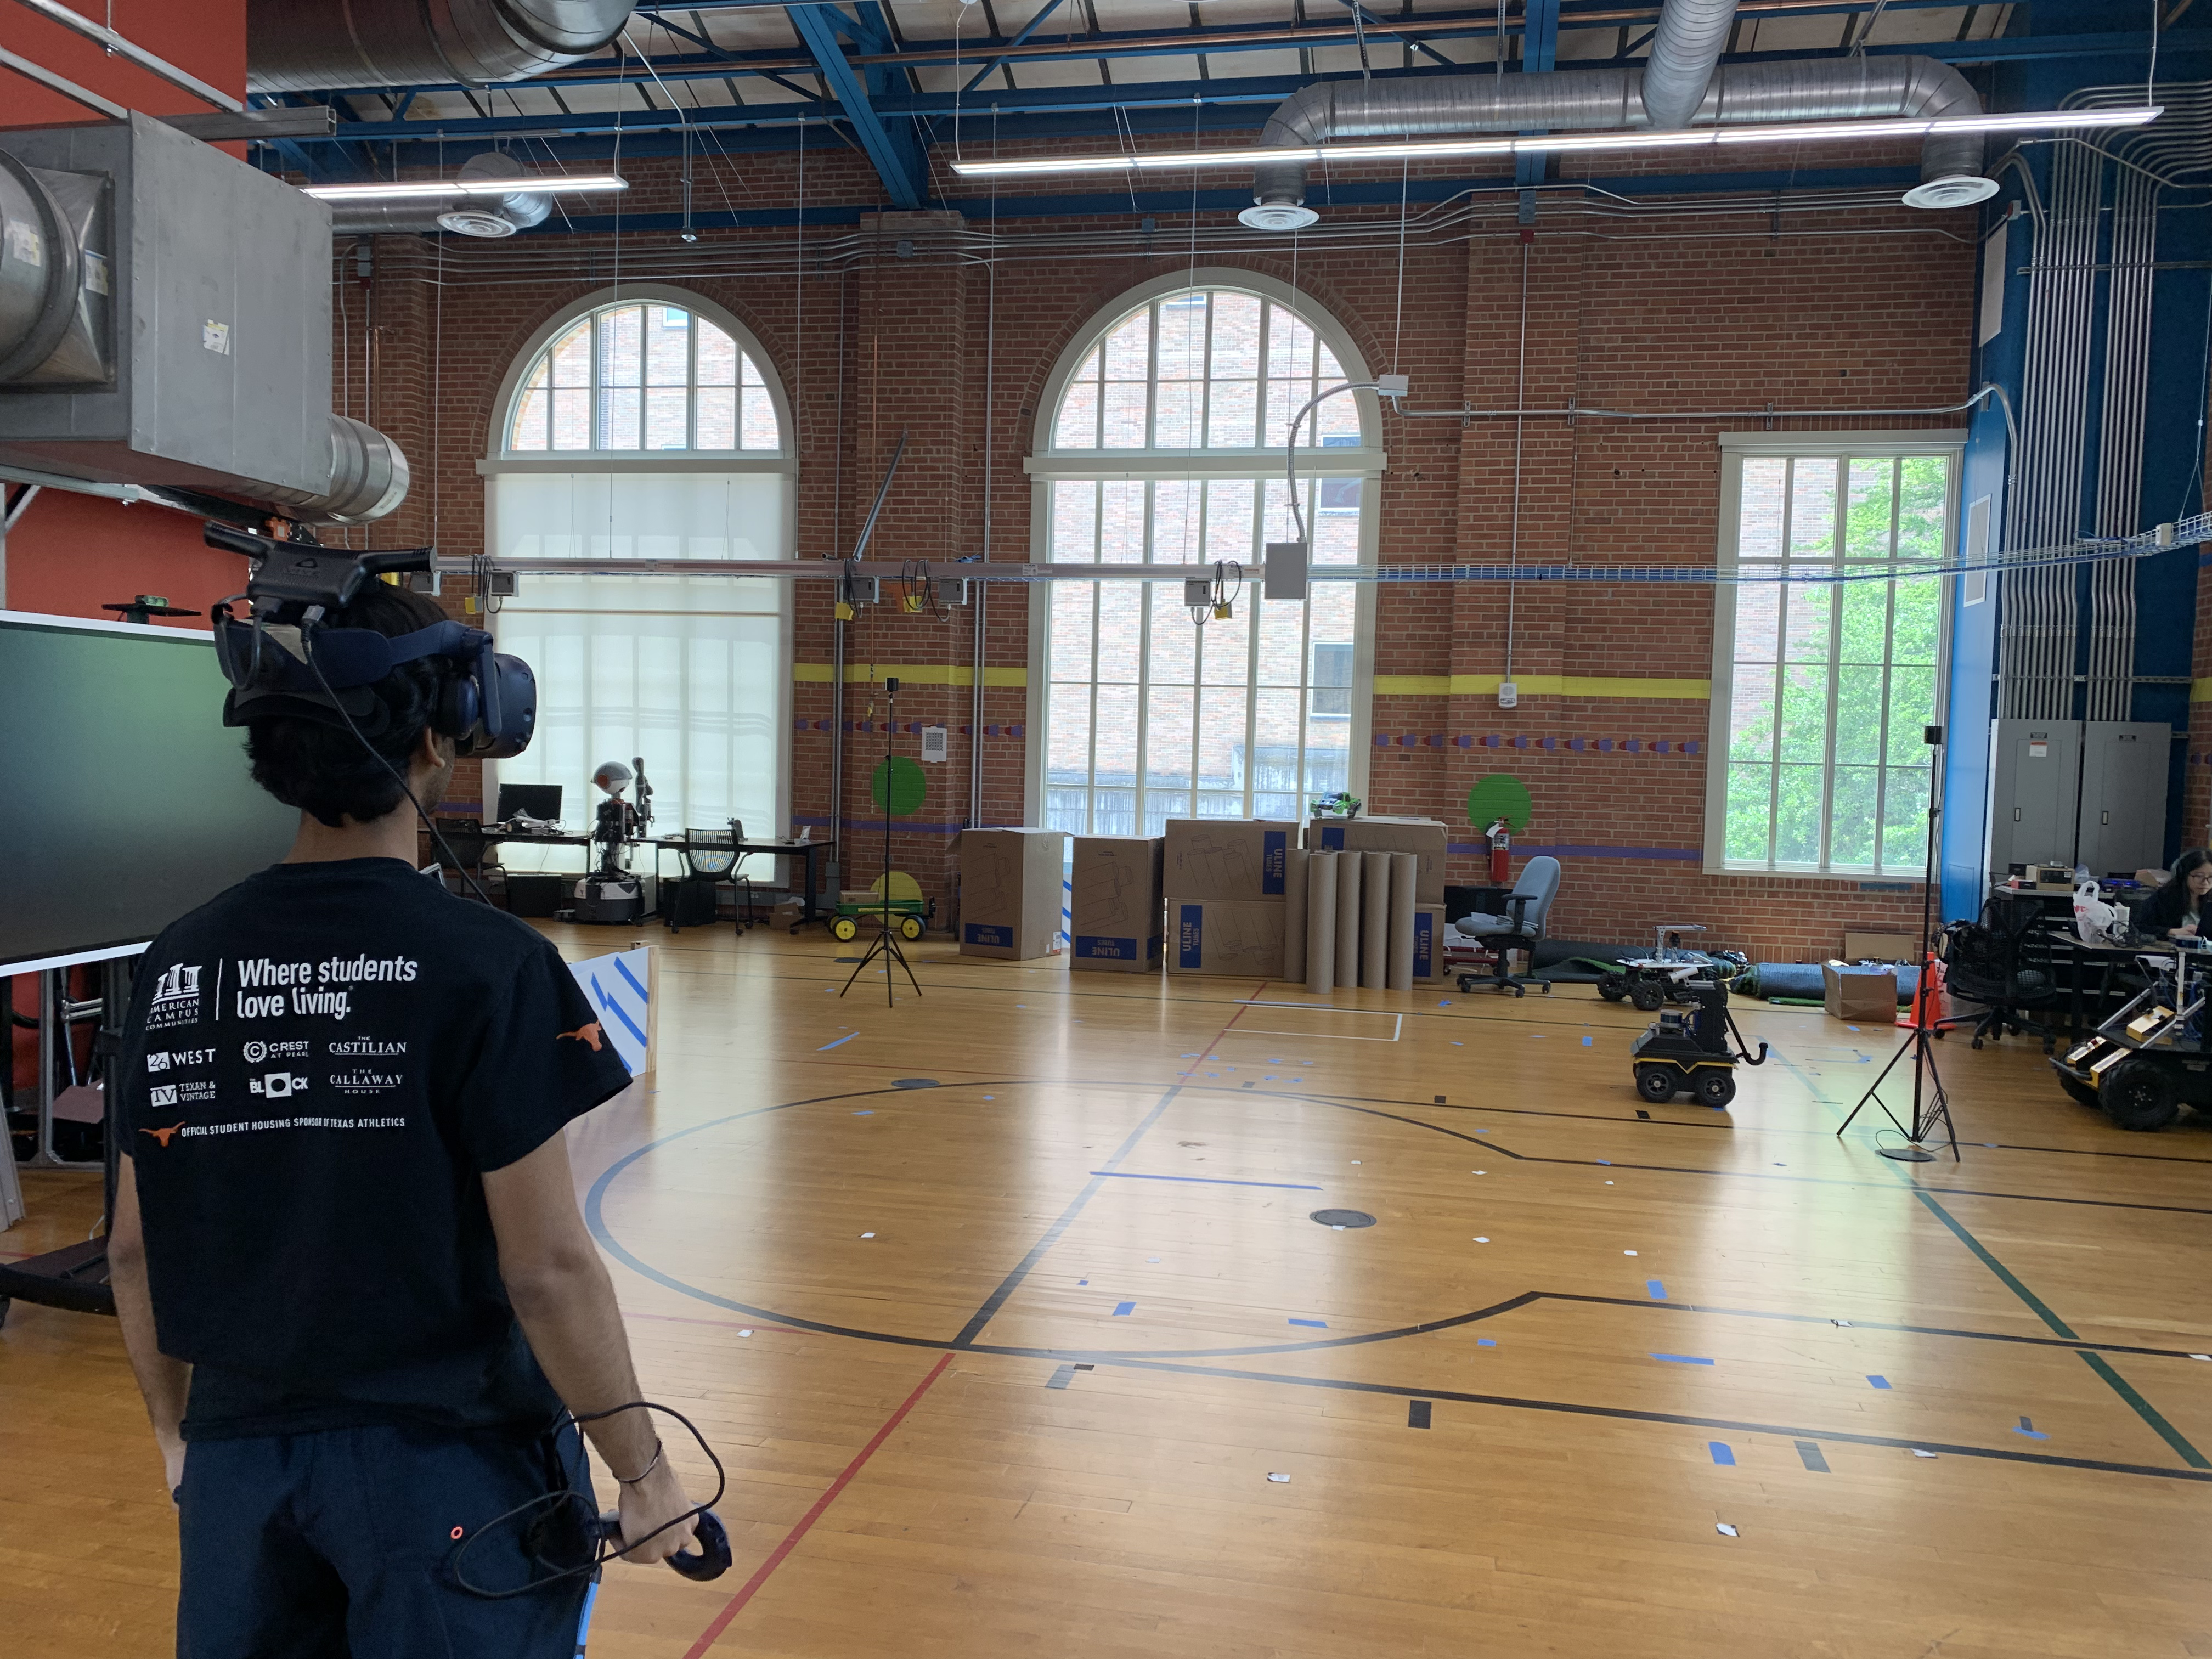
\includegraphics[scale=0.063]{IRL Perspective.png}
\caption{Participant's outside environment view while wearing a HTC Vive Pro Eye headset and holding the two Vive controllers. The controllers are not used by the participant but are used to calibrate the user's position in the space.}
\end{figure}

\section{Discussion}
Our findings show that head orientation predetermines direction as participants were looking in the direction they were walking. This allows the robot to intercept their path by focusing on their head orientation. In work settings, humans tend to focus their attention on threats [10], such as the robot's appearance. So if a person focuses their attention on the robot while walking sideways to avoid the obstacle, they manage to divert the robot, as seen in the trials. Thus, a real-world application of a blocking robot should utilize head orientation to predict a person's movements only to a certain extent. To accurately block a person, the robot should follow the head orientation until a certain angle is reached to prevent the robot from being at the side of the person instead of in front of them. 

\section{Conclusion}

For robots to coexist with humans, social navigation is required to ensure the safety of both man and machine. Previous research has included using position and velocity to anticipate movement [2], but head orientation [3] is a better indicator in free-range environments with unanticipated stimuli. Our research further reinforces that a person's head orientation will foreshadow their direction. While this study provides a strong backbone between head orientation and movement of people, the more significant and unique purpose was to identify the interaction humans have when targeted and followed by autonomous robots. 

This study clearly showed users a change of pace and approach to the virtually simulated hallway upon the understanding that the robot was trying to target them, unlike before. While participants continued to try to reach the end of the hallway (as instructed), there was a clear shocked and confused reaction within a few seconds of starting the fourth trial. This result strongly indicates the positive use of robots in coexisting environments with people as we can implement tracking algorithms knowing that humans will understand that the robot is trying to block/follow them. 

%%%%%%%%%%%%%%%%%%%%%%%%%%%%%%%%%%%%%%%%%%%%%%%%%%%%%%%%%%%%%%%%%%%%%%%%%%%%%%%%

\begin{thebibliography}{99}

\bibitem{c1} 
Kivrak, H., Cakmak, F., Kose, H., \& ; Yavuz, S. (2020, September 3). Social Navigation Framework for assistive robots in human inhabited unknown environments. Engineering Science and Technology, an International Journal. Retrieved May 11, 2022, from https://www.sciencedirect.com/science/article/pii/S2215098620308727 


\bibitem{c2}
Holman, B., Anwar, A., Singh, A., Tec, M., Hart, J.W., \& Stone, P. (2021). Watch Where You’re Going! Gaze and Head Orientation as Predictors for Social Robot Navigation. 2021 IEEE International Conference on Robotics and Automation (ICRA), 3553-3559.

\bibitem{c3}
Zeng L, Bone GM. Mobile Robot Collision Avoidance in Human Environments. International Journal of Advanced Robotic Systems. January 2013. doi:10.5772/54933


\bibitem{c4}
Herry, C., Bach, D. R., Esposito, F., Di Salle, F., Perrig, W. J., Scheffler, K., Lüthi, A., \& Seifritz, E. (2007). Processing of temporal unpredictability in human and animal amygdala. The Journal of neuroscience : the official journal of the Society for Neuroscience, 27(22), 5958–5966. https://doi.org/10.1523/JNEUROSCI.5218-06.2007

\bibitem{c5} 
Nummenmaa, L., Hyönä, J., \& Hietanen, J. K. (2009). I'll walk this way: eyes reveal the direction of locomotion and make passersby look and go the other way. Psychological science, 20(12), 1454–1458. https://doi.org/10.1111/j.1467-9280.2009.02464.x
  
\bibitem{c6}
“Vive Pro Eye Series,” https://www.vive.com/eu/product/vive-pro-
eye/overview/, Accessed: 2022-04-10.

\bibitem{c7}
Hollands, M. A., Patla, A. E., \& Vickers, J. N. (2002). "Look where you're going!": gaze behaviour associated with maintaining and changing the direction of locomotion. Experimental brain research, 143(2), 221–230. https://doi.org/10.1007/s00221-001-0983-7

\bibitem{c8}
Lichtenthäler, C., Peters, A., Griffiths, S., \&; Kirsch, A. (1970, January 1). Social Navigation - identifying robot navigation patterns in a path crossing scenario. SpringerLink. Retrieved May 9, 2022, from https://link.springer.com/chapter/10.1007/978-3-319-02675-6

\bibitem{c9} 
O. Liu, D. Rakita, B. Mutlu and M. Gleicher, "Understanding human-robot interaction in virtual reality," 2017 26th IEEE International Symposium on Robot and Human Interactive Communication (RO-MAN), 2017, pp. 751-757, doi: 10.1109/ROMAN.2017.8172387. 

\bibitem{c10}
Ford, B. Q., Tamir, M., Brunyé, T. T., Shirer, W. R., Mahoney, C. R., \& Taylor, H. A. (2010). Keeping Your Eyes on the Prize: Anger and Visual Attention to Threats and Rewards. Psychological Science, 21(8), 1098–1105. http://www.jstor.org/stable/41062340

\bibitem{c11}
Technologies, U. (n.d.). Unity. Retrieved May 11, 2022, from https://unity.com/, Accessed: 2022-04-10.

\bibitem{c12}
Foundation, B. (n.d.). Home of the blender project - free and open 3D creation software. blender.org. Retrieved May 11, 2022, from https://www.blender.org/, Accessed: 2022-04-10.

\bibitem{c13}
Valve corporation. SteamVR. (n.d.). Retrieved May 11, 2022, from https://www.steamvr.com/en/, Accessed: 2022-04-10.

\bibitem{c14}
OBS Studio. OBS. (n.d.). Retrieved May 11, 2022, from https://obsproject.com/, Accessed: 2022-05-09.

\end{thebibliography}

\end{document}
